\documentclass{article}
\usepackage[utf8]{inputenc}
\title{Lab 2:Gradient Descent and Stochastic Gradient Descent}
\author{wbg231 }
\date{December 2022}
\newcommand{\R}{$\mathbb{R}$}
\newcommand{\B}{$\beta$}
\newcommand{\A}{$\alpha$}
\newcommand{\D}{\Delta}

\newcommand{\avector}[2]{(#1_2,\ldots,#1_{#2})}
\newcommand{\makedef}[2]{$\textbf{#1}$:#2 }
\usepackage{tikz,graphicx,hyperref,amsmath,amsfonts,amscd,amssymb,bm,cite,epsfig,epsf,url}

\begin{document}

\maketitle

\section{introduction}
\begin{itemize}
\item \href{https://nyu-ds1003.github.io/mlcourse/2023/labs/Lab2.pdf}{slides} 
\item this starts off with a review of gradient descent I am going to skip that since, the notes i took in lecture 2 on the material were pretty thorough. 
\section{gradient descent learning rate}
\itme suppose we want to find $\theta^{*}\in \mathbb{R}$ that minimizes $f(\theta)=\that^2-2\theta+1$
\item this is a problem we can easily solve analytically but lets see how gradient descent does 
\item 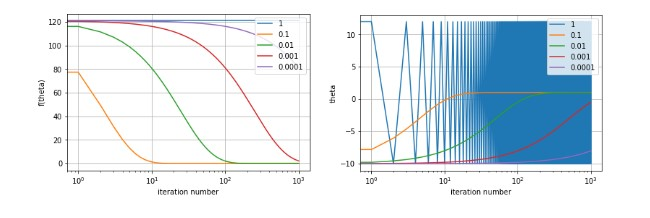
\includegraphics[width=10cm]{labs/lab_2/immages/lab_2_1.jpg}
\item we can see here that $\alpha=1$ does not lead to convergence. 
\itme while an $\alpha$ that is to small makes converge take a really long time so we want a good middle ground 
\subsection{adaptive learning rate}
\item instead of a fixed learning rate we can adjust our learning rate each iteration 
\item example algorithm 
\begin{itemize}
    \item at each iteration of i 
    \begin{itemize}
        \item $\Tilde{\theta}=\theta_{i-1}-\epsilon_{i-1}\nabla f(\theta_{i-1})$ so typical gradient descent update 
        \item $\delta=f(\theta_{i-1}-f(\Tilde{\theta})$ so find how much our loss function has changed 
        \item if $\delta\geq $ threshold
        \begin{itemize}
            \item we are happy with our reduction in loss 
            \item $\theta_i=\Tilde{\theta}$ we update our $theta$
            \item we increase the learning rate next iteration $\epsilon_{j}=2\epsilon_{j+1}$
        \end{itemize}
        \item else
        \begin{itemize}
            \item we are not happy with the reduction in our loss function 
            \item $\theta_{i}=\theta_{i-1}$ ie keep $\theta$ the same as last iteration
            \itme we reduce the learning rate $\epsilon_{j}=\frac{1}{2}\epsilon_{j-1}$
        \end{itemize}
    \end{itemize}
\end{itemize}
\item how to make a proper threshold $f(\theta_{i-1})-f(\Tilde{\theta})$?
\subsection{armijo rule}
\item we can use  armijo rule 
\item  if the learning rate $\alpha$ satisfies $$f(\theta_{i-1}-f(\Tilde{\theta})\geq \frac{1}{2}\alpha||\nabla f(\theta_{i-1})||^2$$ then $f(\theta)$ will converge to a local min
\item this tells us that if our learning rate satisfies this condition, we can set our threshold in a way that will guarantee  we end up with a local min for our risk function. 
\section{Stochastic gradient descent }
\item Stochastic gradient descent algo
\begin{itemize}
    \item initialize w
    \item repeat until stopping condition 
    \begin{itemize}
        \item chose a single training point from the data set $(x_i,y_i)\in D_n$
        \item $x\leftarrow w-\alpha \nabla_{W}\ell(f_{w}(x_i),y_i)$ ie take the grad loss on the ith example 
    \end{itemize}
    \item this is equiv lent to mini batch gradient descent with bath size $n=1$
\end{itemize}
\section{gradient descent for linear regression }
\item input space $X=\mathbb{R}^{d}$ output space $y=\mathbb{R}$
\item data: input are features vectors outputs are scalars $D=\{x_i,y_i\}_{i=1}^{n}$
\item hypothesis space. $\mathcal{F}=\{f:\mathbb{R}^{d}\rightarrow \mathbb{r}|f(x)=\theta^tx, \theat \in \mathbb{R}^{d}\}$ 
\item action our prediction is a leaner function of the inputs
\item we use square loss $\ell(\hat{y},y)=(y-\hat{y})^2$
\item goal find the set of parameters that minimize the empirical risk $\hat{R}_{n}(\theta)=\frac{1}{n}\Sigma_{i=1}^{n}(\theta^{t}x_{i}-y_i)^2$
\item call our loss function $J(\theta)=\frac{1}{2}\Sigma_{i=1}^{n}(\theta^{t}x_i-y_i)^2$  this will have the same arg min as risk, but the $\frac{1}{2}$ will have an derivative.
\item three approach's
\subsection{approach 1: closed form solution}
$J(\theta)=\frac{1}{2}\Sigma_{i=1}^{n}(\theta^{t}x_i-y_i)^2=\frac{1}{2}(\theta^{t}X-y)^{t}(\theta^{t}X-y)=\frac{1}{2}||X\theta-y||_{2}^{2}$
\item then we can see that $\nabla j(\theta)=(X^TX\theta-X^ty)=X^t(X\theta-y)=0\Rightarrow \hat{\theta}=(X^{t}X)^{-1}X^{T}y$
\item this is nice because it is one shot
\item this does not scale well however because matrix inverse are expensive
 \end{itemize}
\item the two other approaches are gradient descent and stochastic gradient descent they are really just running the algos we already have
 \section{gradient descent for logistic regression }
\item inputs are feature vectors of dimension d targets are class labels 0,1
\item action our predicting is the probability of class label given linear signals $h_{\theta}(x)=\frac{1}{1+e^{-\theta^{t}x}}$
\item call $P(y=1|x,\thea)=h_{\theta}(x)$ and$P(y=0|x,\thea)=1-h_{\theta}(x)$ 
\item we assume that $(x_1,y_1)...(x_n,y_n)$ are iid 
\item we define the likely hood as as $P(y_1\cap y_2...\cap y_n|x_1\cap x_2...\cap x_n)=P(y_1|x_1,\theta)P(y_2|x_2\theta)...P(y_n|x_n\theta)=\Pi_{i=1}^{n}=\Pi_{i=1}^{n}P(y=1|x,\theta)(1-P(y=1|x,\theta))=\Pi_{i=1}^{n}h_{\theta}(x_i)^{y_i}(1-h_{\theta}(x_i))^{1-y_i}$ 
\item so our goal is to minimize the log likelihood $\ell(\theta)=log(L(\thea))=\Sigma_{i=1}^{n}y_ilogh_{\theta}(x_i)+(1-y_i)log(1-h_{\theta}(x_i))$ where $y_i$ is the number of positive classes.
\item this logistic loss does not have a analytic solution 
\item so we can use gradient ascent which is just gradient descent but with the update rule $\theta=\thea+\alpha \nabla_{\theta}\ell)$
 
\end{document}
